\documentclass[12pt]{article}
\usepackage[utf8]{inputenc}
\usepackage[margin=1in,left=1.5in,includefoot]{geometry}
\usepackage{booktabs}
\usepackage[english, greek]{babel}
\newcommand{\en}[1]{\foreignlanguage{English}{#1}}
\usepackage{graphicx}
\usepackage{subcaption}

 
% Header & Footer Stuff

\usepackage{fancyhdr}
\pagestyle{fancy}
\lhead{Εκπαιδευτικό Λογισμικό 2024}
\fancyfoot{}
\fancyfoot[R]{}

% The Main Document
\begin{document}

\begin{center}
 \LARGE\bfseries \en{Learning Python}
 \line(1,0){430}
\end{center}


\newline

 Για την εργασία μας, επιλέξαμε να δημιουργήσουμε ένα εκπαιδευτικό λογισμικό για την εκμάθηση της γλώσσας προγραμματισμού \en{Python} . Η ανάπτυξη της εφαρμογής έγινε με τη χρήση \en{Windows Forms} και προγραμματίστηκε σε \en{C\#}.

\section*{\en{Login}}
\begin{center}
    
    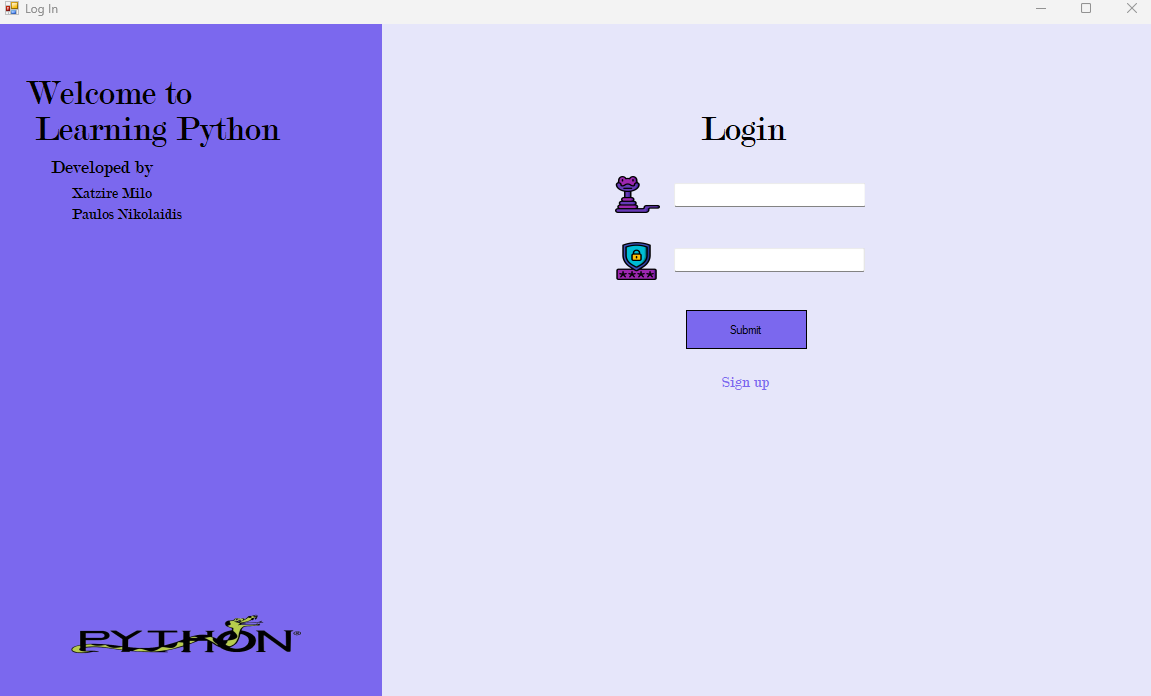
\includegraphics[width=1.1\linewidth]{login.png}
\end{center}

Μόλις ανοίξουμε την εφαρμογή, υπάρχει η δυνατότητα σύνδεσης και η δυνατότητα εγγραφής σε περίπτωση που είναι καινούριος χρήστης.Τα στοιχεία αποθηκεύονται στην βάση, την οποία θα αναλύσουμε στην συνέχεια. Πραγματοποιείται έλεγχος των στοιχείων.


 
\begin{figure}
  \centering
  \begin{subfigure}{0.38\textwidth}
    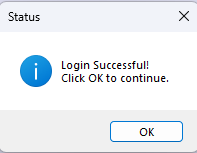
\includegraphics[width=\linewidth]{loginmsg.png}
    \caption{Επιτυχής Σύνδεση}
    \label{fig:subfig1}
  \end{subfigure}
  \hfill
  \begin{subfigure}{0.45\textwidth}
    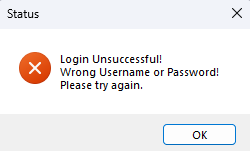
\includegraphics[width=\linewidth]{msgloginerror.png}
    \caption{Εσφαλμένη Συμπλήρωση Στοιχείων}
    \label{fig:subfig2}
  \end{subfigure}

  \label{fig:two_images}
\end{figure}

\section*{\en{Sign Up}}

\begin{center}

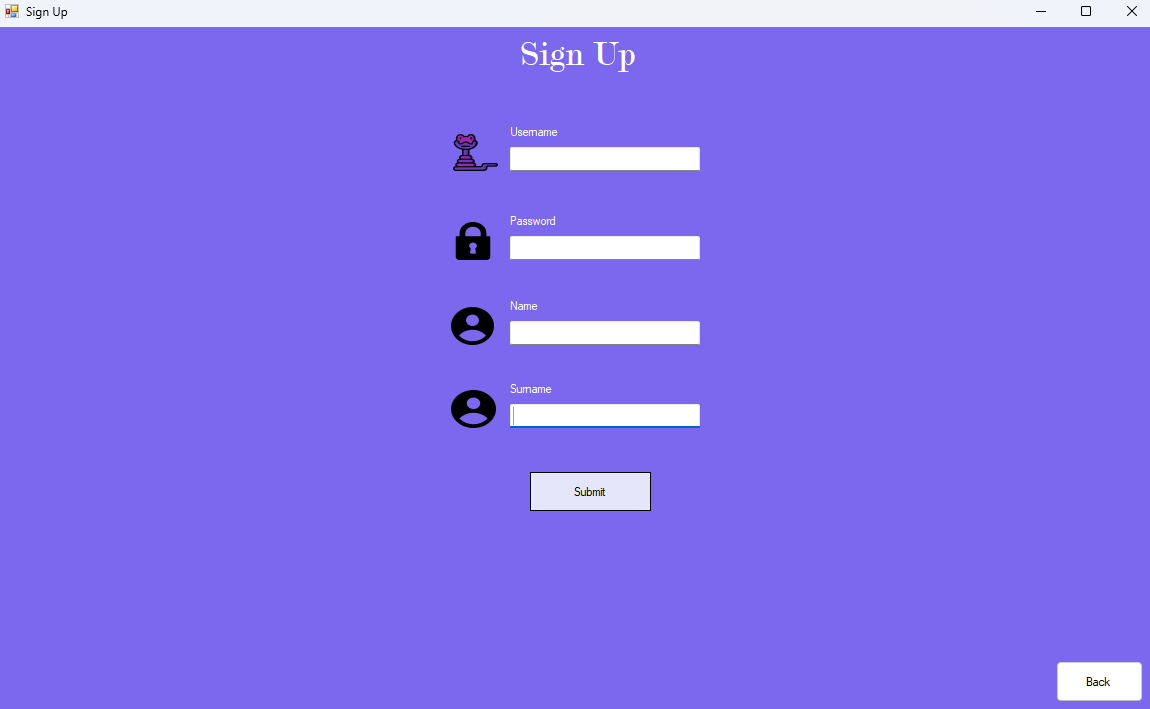
\includegraphics[width=1\linewidth]{signup.png}

\end{center}

Για να εγγραφεί ο χρήστης πρέπει να συμπληρώσει \en{Username, Password, Name} και \en{Surname}.
Πραγματοποιείται έλεγχος ώστε τα πεδία να μην είναι κενά και το \en{Username} να είναι μοναδικό.

\begin{figure}
  \centering
  \begin{subfigure}{0.32\textwidth}
    
\includegraphics[width=\linewidth]{signupmsg.png}
    \caption{Επιτυχής Εγγραφή}
    \label{fig:subfig1}
  \end{subfigure}
  \hfill
  \begin{subfigure}{0.53\textwidth}
    
\includegraphics[width=\linewidth]{signuperrormsg.png}
    \caption{Εσφαλμένη Συμπλήρωση Στοιχείων}
    \label{fig:subfig2}
  \end{subfigure}

  \label{fig:two_images}
\end{figure}
\newpage
\section*{\en{Menu}}

Μολίς πραγματοποιηθεί η σύνδεση, ο χρήστης κατευθύνεται στο μενού όπου εμφανίζονται τα κεφάλαια και το κουιζ κάθε κεφαλαίου.Δεξιά βλέπουμε τα βασικά κεφάλαια και αριστερά τα προχωρημένα.Στο πάνω μέρος της φόρμας εμφανίζονται τα \en{clicks} που έχει κάνει ο χρήστης στα κεφάλαια, ο συγκεκριμένος χρήστης ήταν καινούριος για αυτό βλέπουμε "\en{No clicks found for the user".} Στο κάτω μέρος υπάρχει το \en{username} του χρήστη και στα δεξιά υπάρχει δυνατότητα αποσύνδεσης.

\begin{center}
    
    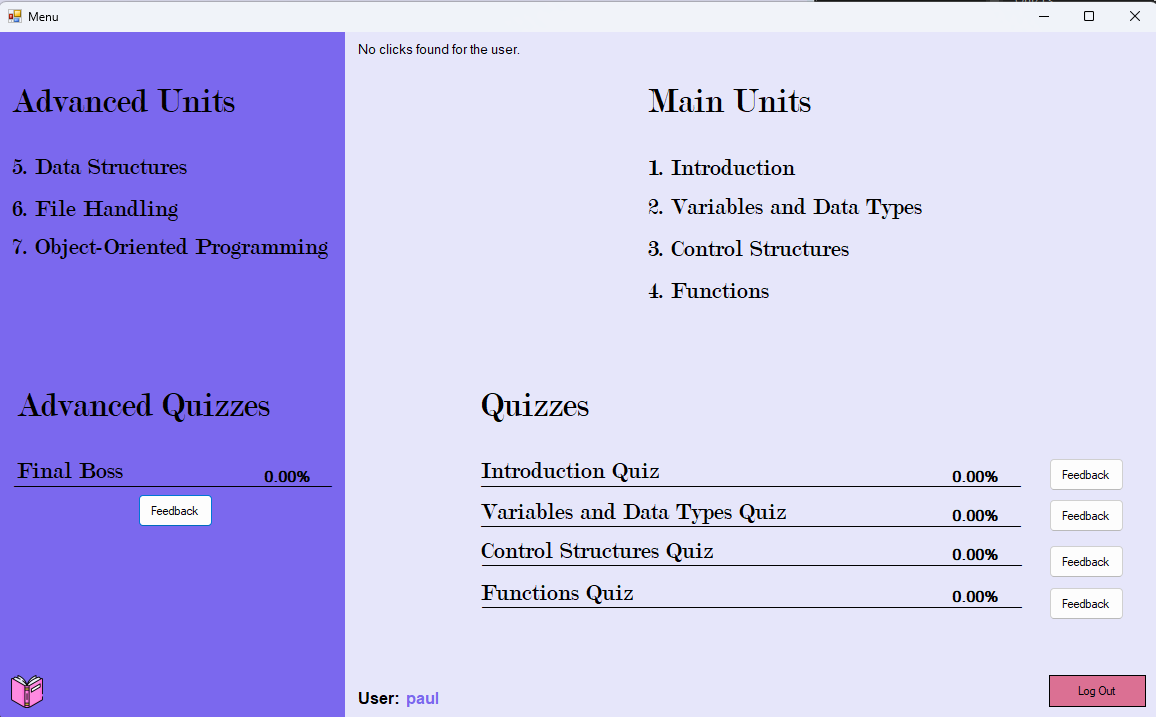
\includegraphics[width=1\linewidth]{image.png}
\end{center}
\newpage
\section*{\en{Unit Forms}}
Μόλις ο χρήστης πατήσει κάποιο κεφάλαιο, εμφανίζεται το παρακάτω μενού με όλες τις υποενότητες του κεφαλαίου.
Σε όλες τις φόρμες θεωρίας , ο χρήστης μπορεί εύκολα να επιστρέψει στην προηγούμενη σελίδα με το κουμπί \en{Back}.
\begin{center}
    
    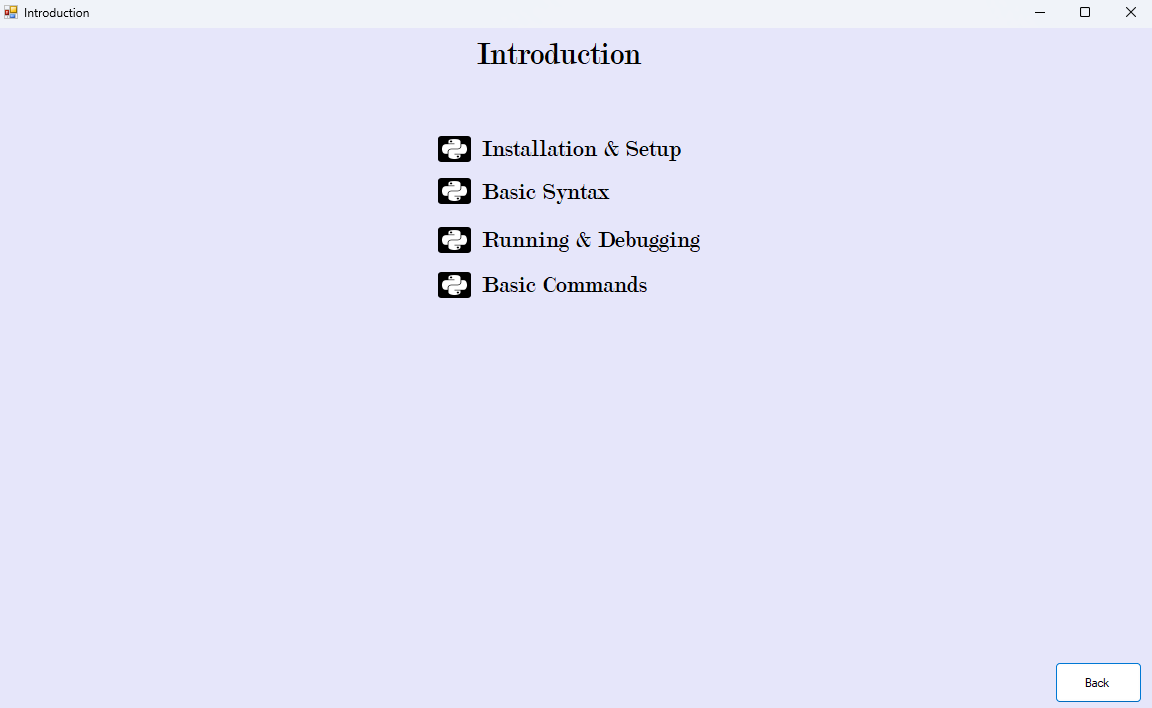
\includegraphics[width=1\linewidth]{unitmenu.png}
\end{center}
\subsection*{\en{Subunit Forms}}
\begin{center}
    
    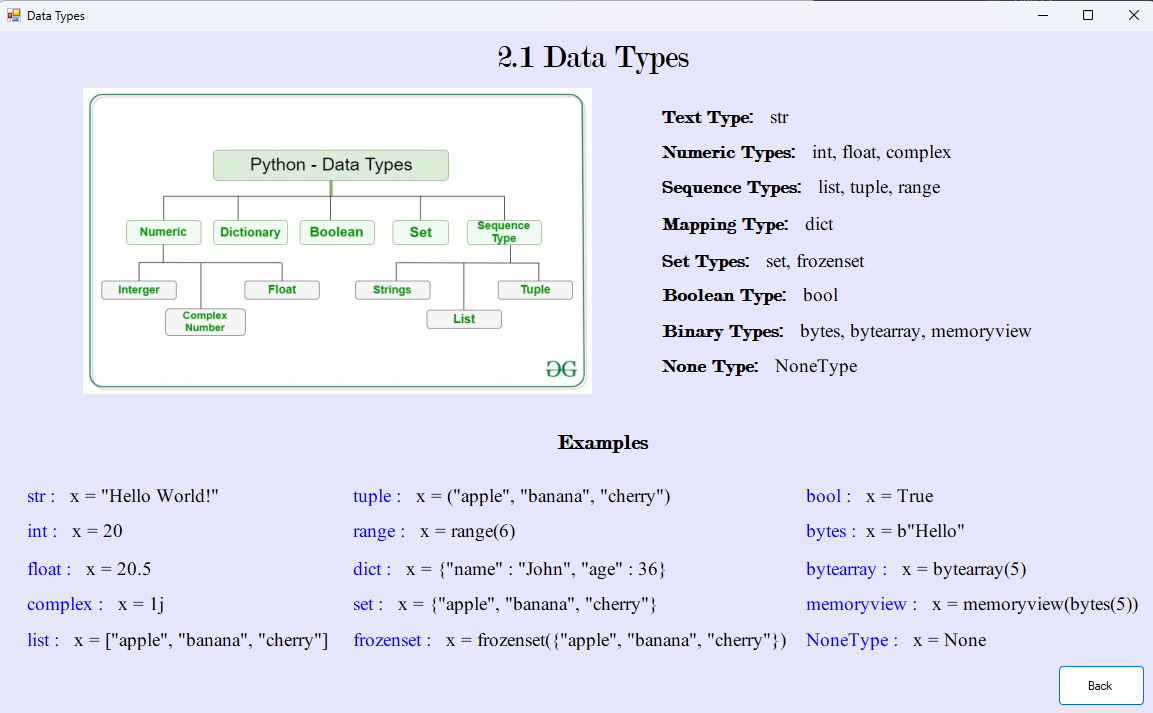
\includegraphics[width=1\linewidth]{subunit.png}
\end{center}

\section*{\en{Quiz Forms}}
Για κάθε βασικό κεφάλαιο υπάρχει 1 κουιζ με 10 ερωτήσεις , τα προχωρημένα κεφάλαια συνδυάζονται σε 1 κουιζ με 10 ερωτήσεις.
Αφού ο χρήστης ολοκληρώσει κάποιο κουιζ, στο Μενού εμφανίζεται το ποσοστό επιτυχίας του και ακριβώς δίπλα υπάρχει το κουμπί \en{Feedback} που εμφανίζει στον χρήστη τις ερωτήσεις που απάντησε λάθος και τις υποενότητες στις οποίες πρέπει να ανατρέξει για να διορθώσει τα λάθη του.
\newpage
Παράδειγμα κουιζ:
\begin{center}

    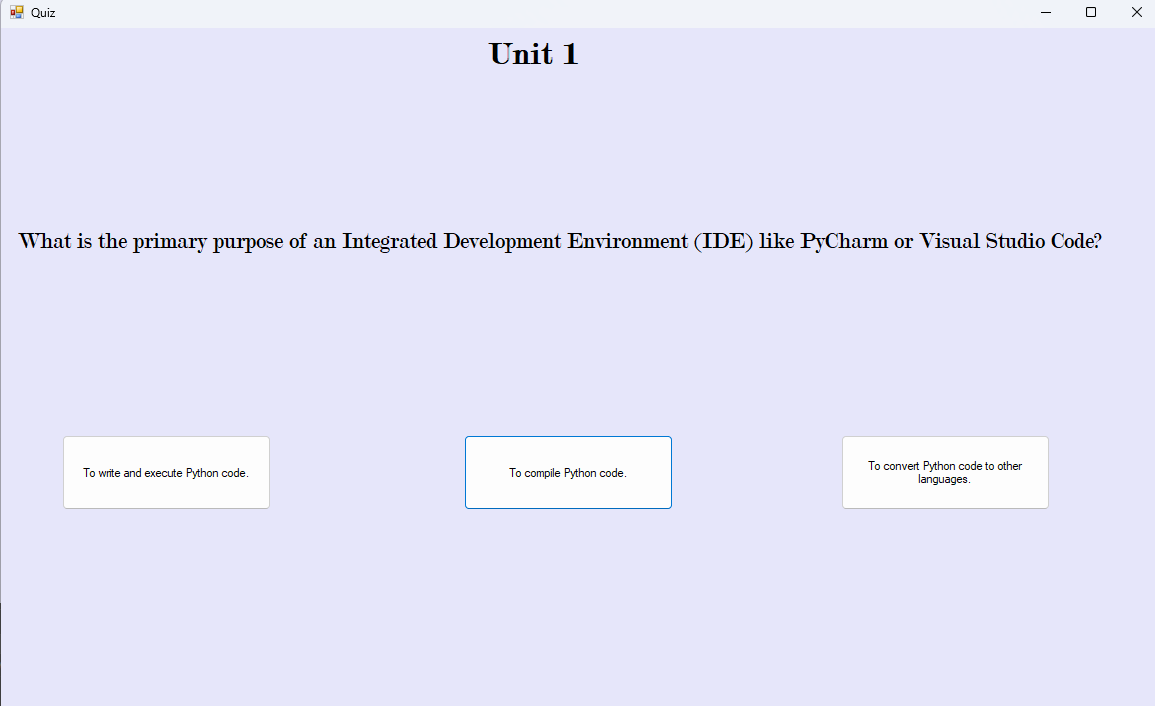
\includegraphics[width=1\linewidth]{quizform.png}
\end{center}
Τα ενημερωμένα ποσοστά αφού ο χρήστης έκανε τα κουιζ:
\begin{center}
    
    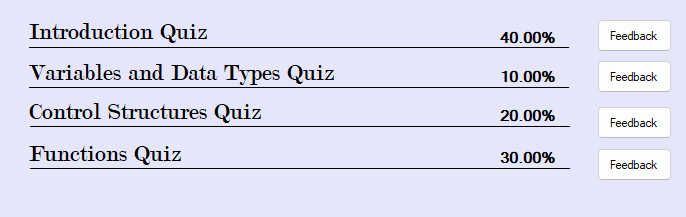
\includegraphics[width=0.8\linewidth]{pososta.png}
\end{center}
\newpage
Τα λάθη του χρήστη και οι προτάσεις διαβάσματος:
\begin{center}
    \
    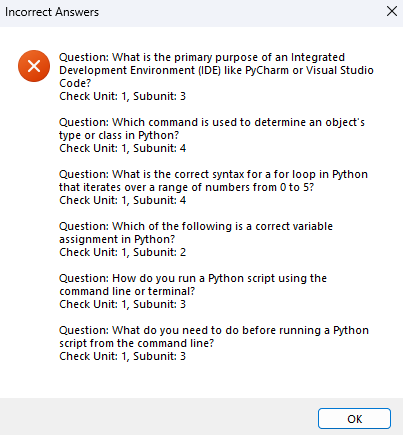
\includegraphics[width=0.8\linewidth]{mistakes.png}
\end{center}
\newpage
\section*{\en{Database}}

Για την βάση δεδομένων της εργασίας χρησιμοποιήσαμε \en{Microsoft Sql Server}.
Δημιουργήσαμε 5 πίνακες:

\subsection*{\en{Clicks}}

Ο πίνακας \en{Clicks} περιλαμβάνει \en{Username, UnitID, SubunitID, Clicks}.

\begin{center}
    
    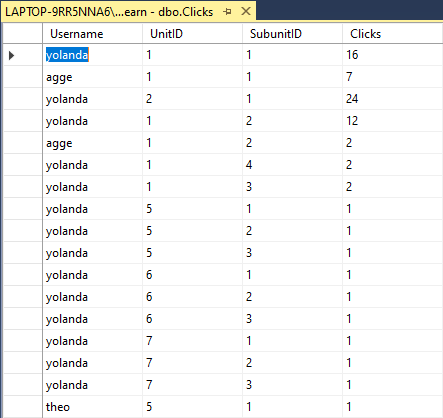
\includegraphics[width=0.7\linewidth]{clicksdb.png}
\end{center}

Ο συγκεκριμένος πίνακας χρησιμοποιείται στην φόρμα \en{Menu} όπου μετρούνται τα \en{clicks}.
Μέσω ενός \en{StringBuilder} συγκεντρώνουμε τα \en{Clicks} για κάθε \en{Unit}.
\newline


Στο πάνω μέρος της σελίδας βλέπουμε τις επισκέψεις του χρήστη στις ενότητες:
\begin{center}
  
    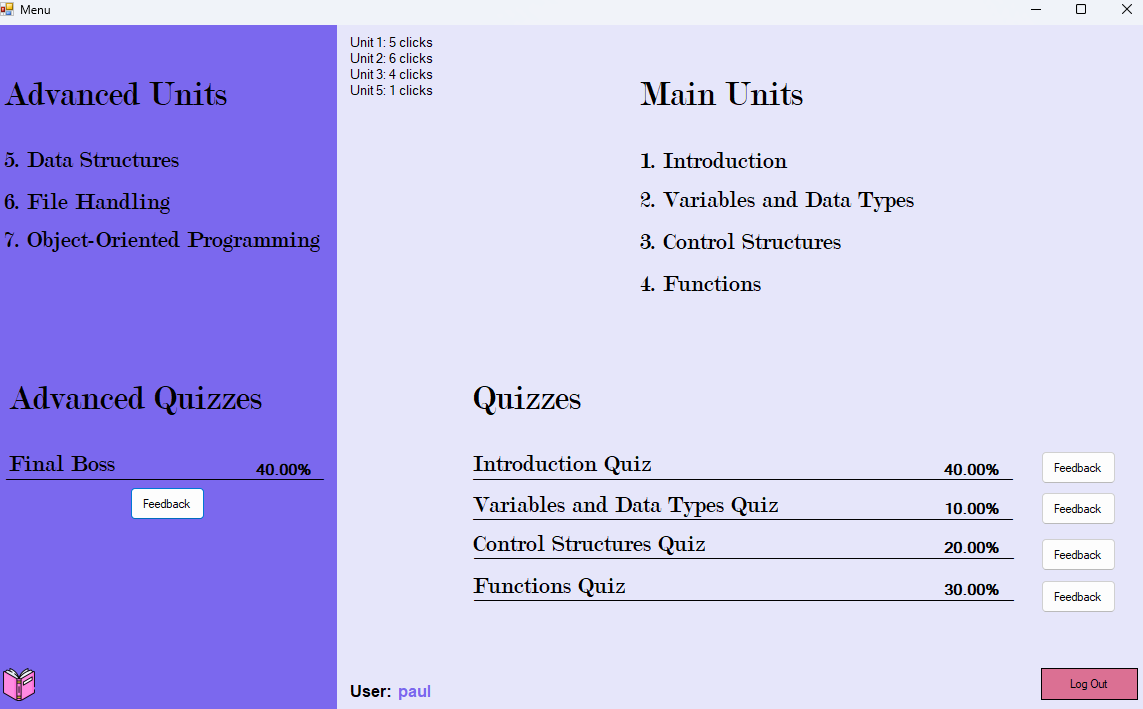
\includegraphics[width=1\linewidth]{clicksexample.png}
\end{center}

\begin{center}
    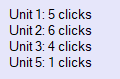
\includegraphics[width=0.5\linewidth]{theclicks.png}
\end{center}




\newpage
\subsection*{\en{Questions}}

Ο πίνακας \en{Questions} περιλαμβάνει \en{QuestionId, QuestionText, UnitID,
\newline
 SubunitID,CorrectAnswerID}.Εκεί έχουμε αποθηκεύσει όλες τις ερωτήσεις των κουιζ.
\begin{center}
    \centering
    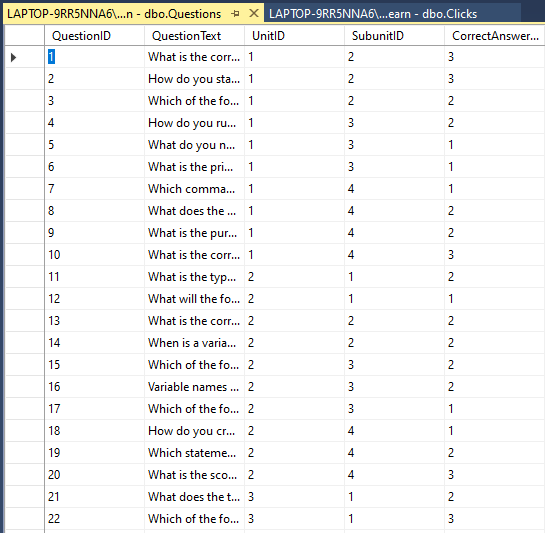
\includegraphics[width=0.8\linewidth]{questionsdb.png}
\end{center}

Χρησιμοποιείται για:
\begin{itemize}
    \item Εμφάνιση των εκφωνήσεων
    \item Έλεγχο Απαντήσεων
\end{itemize}
\newpage

\subsection*{\en{QuestionsAnswers}}

Περιλαμβάνει \en{QuestionID, AnswerID, AnswerText}

\begin{center}
    
    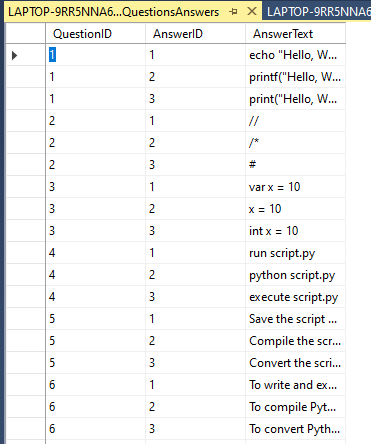
\includegraphics[width=0.8\linewidth]{questionsanswersdb.png}
\end{center}

Χρησιμοποιείται για την εμφάνιση των απαντήσεων στο κουιζ.

\newpage
\subsection*{\en{Users}}

Περιλαμβάνει \en{Username, Password, Name, Surname}.



\begin{center}

    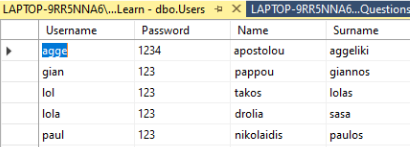
\includegraphics[width=0.8\linewidth]{usersdb.png}
\end{center}


Στον πίνακα \en{Users} αποθηκεύονται τα στοιχεία του χρήστη κατά την εγγραφή και χρησιμοποιείται και για έλεγχο των στοιχείων κατά την σύνδεση.


\subsection*{\en{UsersAnswers}}

Περιλαμβάνει \en{QuestionID, QuizID, Datetime, Username, AnswerID}



\begin{center}
    
    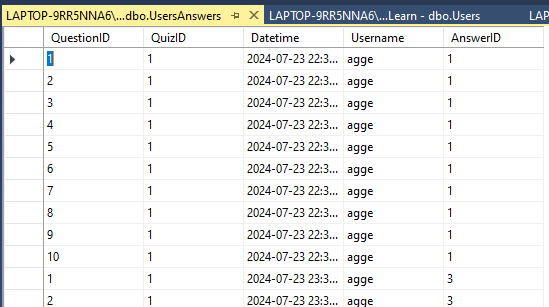
\includegraphics[width=0.8\linewidth]{usersanswersdb.png}
\end{center}


Χρησιμοποιείται σε συνδυασμό με τον πίνακα \en{Questions} για τον έλεγχο των απαντήσεων του χρήστη.

\newpage
 \section*{Πηγές Θεωρίας}

\begin{itemize}
    \item \en{W3schools}
    \item \en{GeeksForGeeks}
    \item \en{Python.org}
\end{itemize}






\end{document}